\documentclass{article}

\usepackage{tikz} 
\usetikzlibrary{automata, positioning, arrows, arrows.meta} 

\usepackage{amsthm}
\usepackage{amsfonts}
\usepackage{amsmath}
\usepackage{amssymb}
\usepackage{fullpage}
\usepackage{color}
\usepackage{parskip}
\usepackage{hyperref}
  \hypersetup{
    colorlinks = true,
    urlcolor = blue,
    linkcolor= blue,
    citecolor= blue,
    filecolor= blue,
    }
    
\usepackage{listings}

\definecolor{dkgreen}{rgb}{0,0.6,0}
\definecolor{gray}{rgb}{0.5,0.5,0.5}
\definecolor{mauve}{rgb}{0.58,0,0.82}

\lstset{frame=tb,
  language=haskell,
  aboveskip=3mm,
  belowskip=3mm,
  showstringspaces=false,
  columns=flexible,
  basicstyle={\small\ttfamily},
  numbers=none,
  numberstyle=\tiny\color{gray},
  keywordstyle=\color{blue},
  commentstyle=\color{dkgreen},
  stringstyle=\color{mauve},
  breaklines=true,
  breakatwhitespace=true,
  tabsize=3
}

\newtheoremstyle{theorem}
  {\topsep}
  {\topsep}
  {\itshape\/}
  {0pt}
  {\bfseries}
  {.}
  {5pt plus 1pt minus 1pt}
  {}
\theoremstyle{theorem} 
   \newtheorem{theorem}{Theorem}[section]
   \newtheorem{corollary}[theorem]{Corollary}
   \newtheorem{lemma}[theorem]{Lemma}
   \newtheorem{proposition}[theorem]{Proposition}
\theoremstyle{definition}
   \newtheorem{definition}[theorem]{Definition}
   \newtheorem{example}[theorem]{Example}
\theoremstyle{remark}    
  \newtheorem{remark}[theorem]{Remark}

\setcounter{tocdepth}{3}
\setcounter{secnumdepth}{3}
  
\title{CPSC-354 Report}
\author{Drew Floyd \\ Chapman University}
\date{\today} 

\begin{document}

\maketitle

\begin{abstract}
This abstract will summarize the report at the end of the semester. For now, this is a placeholder.
\end{abstract}

\tableofcontents

\section{Introduction}\label{intro}
This report documents my learning throughout the course, including weekly homework, notes, and reflections. It is structured week-by-week following the provided template and incorporates diagrams, formal reasoning, and examples written in \LaTeX.

\section{Week by Week}\label{homework}

\subsection{Week 1}

\subsubsection{Notes and Exploration}
(Currently Notes are stored in Google Docs)

\subsubsection{Homework: The MU-Puzzle}
MI $\rightarrow$ MU

\textbf{Rule 1:} If you possess a string whose last letter is \texttt{I}, add \texttt{U}.

\textbf{Rule 2:} Suppose you have \texttt{Mx}, you may add \texttt{Mxx}.

\textbf{Rule 3:} If \texttt{III} occurs in one of the strings, you may make a new string with \texttt{U} in place of \texttt{III}.

\textbf{Rule 4:} If \texttt{UU}, you can drop it.

\vspace{1em}

MI \\
MII $\; Mxx$ \\
MIIII $\; Mxx$ \\
MIIIIIIII $\; Mxx$ \\
MUIIU $\; MIU$ \\
$\varnothing$

\vspace{1em}

MI $\; \rightarrow$ use $Mxx$ rule $\infty$ times \\
MIIII... \\

No matter what Rule you use you will never be able to get 0 Mod3, because I will always be 1 mod 3 or 2 mod 3.

\vspace{1em}

\textbf{Rule 1} does not affect \# of I's. \\
\textbf{Rule 2} does not give 0 mod 3. \\
\textbf{Rule 3} does not solve the problem as removing 3 I's does not change the output of mod3. \\
\textbf{Rule 4} does not change the \# of I's. \\

We can never get rid of all of the I's, 0 mod 3 is not possible. Thus you cannot get MU from MI.

\subsubsection{Questions}
What other invariants (besides mod 3) could be useful for proving impossibility results in rewriting systems?

\subsection{Week 2}

\subsubsection{Notes and Exploration}
(Currently Notes are stored in Google Docs)

\subsubsection{Homework: Rewriting Assignment}
\begin{enumerate}
    \item $A = \{ \}$,\quad $R = \{ \}$

    \begin{center}
      
\begin{tikzpicture}
        \node[circle, draw, minimum size=1cm] (a) {};
      \end{tikzpicture}
    \end{center}
    This diagram is terminating because there are no infinite loops, confluent because all paths lead to the same result, and has a unique normal form as there is only one final state.

\vspace{2em}

    \item $A = \{ a \}$,\quad $R = \{ \}$

    \begin{center}
      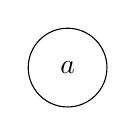
\begin{tikzpicture}
        \node[circle, draw, minimum size=1cm] (a) {$a$};
      \end{tikzpicture}
    \end{center}
    This diagram is terminating because there are no infinite loops, confluent because all paths lead to the same result, and has a unique normal form as there is only one final state.

\vspace{2em}

    \item $A = \{ a \}$,\quad $R = \{ (a,a) \}$

    \begin{center}
      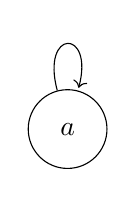
\begin{tikzpicture}
        \node[circle, draw, minimum size=1cm] (a) {$a$};
        \draw[->] (a) edge[loop above] (a);
      \end{tikzpicture}
    \end{center}
    This diagram is not terminating due to the presence of infinite loops, confluent because all paths merge, but does not have a unique normal form as multiple results are possible.

\vspace{2em}

    \item $A = \{ a, b, c \}$,\quad $R = \{ (a,b), (a,c) \}$

    \begin{center}
      \begin{tikzpicture}
        \node[circle, draw, minimum size=1cm] (a) {$a$};
        \node[right=2cm of a, circle, draw, minimum size=1cm] (b) {$b$};
        \node[below=2cm of a, circle, draw, minimum size=1cm] (c) {$c$};
        \draw[->] (a) -- (b);
        \draw[->] (a) -- (c);
      \end{tikzpicture}
    \end{center}
    This diagram is terminating as there are no infinite loops, not confluent because paths diverge, and does not have a unique normal form due to multiple end states.

\vspace{2em}

    \item $A = \{ a, b \}$,\quad $R = \{ (a,a), (a,b) \}$

    \begin{center}
      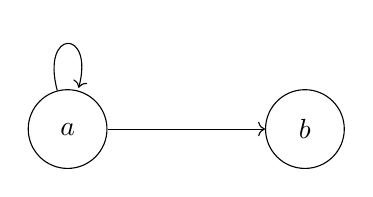
\begin{tikzpicture}
        \node[circle, draw, minimum size=1cm] (a) {$a$};
        \node[right=2cm of a, circle, draw, minimum size=1cm] (b) {$b$};
        \draw[->] (a) -- (b);
        \draw[->] (a) edge[loop above] (a);
      \end{tikzpicture}
    \end{center}
    This diagram is not terminating due to the presence of infinite loops, confluent because all paths lead to b, it has a unique normal form as the single end state is b.

\vspace{2em}

    \item $A = \{ a, b, c \}$,\quad $R = \{ (a,b), (b,b), (a,c) \}$

    \begin{center}
      \begin{tikzpicture}
        \node[circle, draw, minimum size=1cm] (a) {$a$};
        \node[right=2cm of a, circle, draw, minimum size=1cm] (b) {$b$};
        \node[below=2cm of a, circle, draw, minimum size=1cm] (c) {$c$};
        \draw[->] (a) -- (b);
        \draw[->] (a) -- (c);
        \draw[->] (b) edge[loop above] (b);
      \end{tikzpicture}
    \end{center}
    This diagram is not terminating due to the presence of infinite loops, not confluent because paths diverge, and has a unique normal form due to having a single end state on c.

\vspace{2em}

    \item $A = \{ a, b, c \}$,\quad $R = \{ (a,b), (b,b), (a,c), (c,c) \}$

    \begin{center}
      \begin{tikzpicture}
        \node[circle, draw, minimum size=1cm] (a) {$a$};
        \node[right=2cm of a, circle, draw, minimum size=1cm] (b) {$b$};
        \node[below=2cm of a, circle, draw, minimum size=1cm] (c) {$c$};
        \draw[->] (b) edge[loop above] (b);
        \draw[->] (c) edge[loop below] (c);
        \draw[->] (a) -- (b);
        \draw[->] (a) -- (c);
      \end{tikzpicture}
    \end{center}
    This diagram is not terminating due to the presence of infinite loops, not confluent because paths diverge, and does not have a unique normal form due to no end states.
\end{enumerate}

\paragraph{Properties Table.}
\begin{center}
\begin{tabular}{c c c c p{8cm}}
     T & C & U & Example(s) & Explanation \\ \hline
    True & True & True & 1, 2 & These examples terminate, are confluent, and have a unique normal form because all paths lead to a single final state without divergence or loops. \\
    True & False & False & 4 & This example terminates but is not confluent due to diverging paths and does not have a unique normal form as multiple end states exist. \\
    False & True & True & 5 & This example does not terminate because a is a loop, but since it loops on itself it can still be confluent and point to b to result in a unique normal form. \\
    False & True & False & 3 & This example does not terminate but is confluent because all paths merge, though it does not have a unique normal form due to multiple results. \\
    False & False & False & 6, 7 & These examples do not terminate, are not confluent due to diverging paths, and do not have a unique normal form as no single end state exists. \\
\end{tabular}
\end{center}

\subsubsection{Questions}
Can we always predict whether an ARS will have a unique normal form just by inspecting the rules, or do we need to test examples?

\subsection{Week 3}

\subsubsection{Notes and Exploration}
(Currently Notes are stored in Google Docs)

\subsubsection{Homework: String Rewriting Exercise 5 and 5b}
\[
\begin{aligned}
  ab &\to ba \\
  ba &\to ab \\
  aa &\to \varepsilon \\
  b  &\to \varepsilon
\end{aligned}
\]

Rewrite steps for \texttt{abba} and \texttt{bababa}: 
\[
\begin{aligned}
  abba &\to abab \to \infty \\
  abba &\to aaba \to aa \to \varepsilon \\
  baba &\to \infty \\
    \\
  ababa &\to \infty \\
  bababa &\to aaba \to aa \to a \\
  bababa &\to \infty
\end{aligned}
\]

\begin{enumerate}
  \item The ARS is not terminating because there is an infinite loop in the first two rules, as they are inverses of each other.

  \item Two equivalence classes: $b \to \varepsilon$ means $b$’s don’t matter, and $aa \to \varepsilon$ means $a$’s cancel in pairs.  
  Normal forms:  
  Even \# of $a$’s $\;\Rightarrow\; \varepsilon$  
  Odd \# of $a$’s $\;\Rightarrow\; a$

  \item You can make the ARS terminating without changing the equivalence classes by removing one of the rules involved in the loop (either $ab \to ba$ or $ba \to ab$).

  \item Semantic question the ARS can answer: “Is the number of $a$’s even or odd?” This works because the complete invariant is the parity of \# of $a$’s.

  \item If instead $aa \to a$, this changes the question from even-or-odd to:  
  No $a$’s $\Rightarrow \varepsilon$  
  At least one $a$ $\Rightarrow a$
\end{enumerate}

\subsubsection{Questions}
How does the choice of termination rule (e.g., $aa \to \varepsilon$ vs. $aa \to a$) change the kinds of invariants that can be expressed? And what are the applications of this?

\section{Essay (Synthesis)}
(Empty placeholder.)

\section{Evidence of Participation}
(Empty placeholder.)

\section{Conclusion}\label{conclusion}
(Empty placeholder.)

\begin{thebibliography}{99}
\bibitem[BLA]{bla} Author, \emph{Title}, Publisher, Year. Available at: \url{https://example.com}
\end{thebibliography}

\end{document}
